\documentclass[11pt,fleqn]{article} % Default font size and left-justified equations

%\usepackage{standalone}

\usepackage{todonotes}
\usepackage{color}
% use \todo{note} OR \missingfigure{Add my picture here}

\usepackage[top=3cm,bottom=3cm,left=3.2cm,right=3.2cm,headsep=10pt,a4paper]{geometry} % Page margins
\usepackage{xcolor} % Required for specifying colors by name
\definecolor{ocre}{RGB}{243,102,25} % Define the orange color used for highlighting throughout the book


% Font Settings


% SLG commented out


% \usepackage{avant} % Use the Avantgarde font for headings
%\usepackage{times} % Use the Times font for headings
% \usepackage{microtype} %Slightly tweak font spacing for aesthetics
% \usepackage{mathptmx} % Use the Adobe Times Roman as the default text font together with math symbols from the Sym­bol, Chancery and Com­puter Modern fonts


%  \usepackage[scaled=0.90]{couriers} %What is this used for?




% SLG commented out
% \def\thereforesymbol{
% \leavevmode
% \lower0.1ex\hbox{$\cdot$}
% \kern-0.2em\raise0.7ex\hbox{$\cdot$}
% \kern-0.2em\lower0.2ex\hbox{$\cdot$}
% \thinspace}


% \usepackage{CJKutf8}
%For cyrillic characters  (do we have any?)


% slg commented this out:
% \usepackage[OT2,T1]{fontenc}
% \DeclareSymbolFont{cyrletters}{OT2}{wncyr}{m}{n}
% \DeclareMathSymbol{\Sha}{\mathalpha}{cyrletters}{"58}


\usepackage[T1]{fontenc}
\usepackage[section]{placeins}

% slg commented these out:
% \usepackage{amssymb}
 \usepackage{fancyvrb}
%  \usepackage{color}




%define a verbatim text for bold user input
\newcommand\verbbf[1]{\textbf{$\blacksquare$ #1}}
%define a verbatim text without box in front
\newcommand\verbbnbf{\textbf}


\PassOptionsToPackage{hyphens}{url}


\usepackage[pdftitle={Users Manual for the hashdb toolset},
              pdfauthor={Bruce Allen, Jessica R. Bradley, Simson L. Garfinkel},
              pdfkeywords={hashdb, block hash database}]{hyperref}
\makeatletter
\g@addto@macro{\UrlBreaks}{\UrlOrds}
\makeatother
% \usepackage{microtype} % Slightly tweak font spacing for aesthetics
%\usepackage[utf8]{inputenc} % Required for including letters with accents
\usepackage[T1]{fontenc} % Use 8-bit encoding that has 256 glyphs




%\usepackage[a4paper,pdftex]{geometry}                                                                                % A4paper margins
\setlength{\oddsidemargin}{5mm}                                                                                                % Remove 'twosided' indentation
\setlength{\evensidemargin}{5mm}


\usepackage[english]{babel}
%\usepackage[protrusion=true,expansion=true]{microtype}        
\usepackage{amsmath,amsfonts,amsthm,amssymb}
\usepackage{graphicx}


\usepackage{tabularx}


% Simson commented this out:
%use autoref or Autoref for lowercase or uppercase beginning of references
\usepackage{catoptions}
\makeatletter
\def\figureautorefname{figure}
\def\tableautorefname{table}
\def\Autoref#1{%
  \begingroup
  \edef\reserved@a{\cpttrimspaces{#1}}%
  \ifcsndefTF{r@#1}{%
    \xaftercsname{\expandafter\testreftype\@fourthoffive}
      {r@\reserved@a}.\\{#1}%
  }{%
    \ref{#1}%
  }%
  \endgroup
}
\def\testreftype#1.#2\\#3{%
  \ifcsndefTF{#1autorefname}{%
    \def\reserved@a##1##2\@nil{%
      \uppercase{\def\ref@name{##1}}%
      \csn@edef{#1autorefname}{\ref@name##2}%
      \autoref{#3}%
    }%
    \reserved@a#1\@nil
  }{%
    \autoref{#3}%
  }%
}
\makeatother


\usepackage{amsmath}


\usepackage{booktabs}


% slg commented out:
% \usepackage{makecell}


\usepackage{color}
\usepackage{graphicx}
%\usepackage {hyperref}
\usepackage{listings}
\usepackage{xspace}


% slg commented out:
\usepackage[toc, page]{appendix}
\usepackage[labelfont=bf]{caption}
%http://tex.stackexchange.com/questions/27663/using- bold-italic-text-inside-listings


% slg commented out:
% \usepackage{multirow} %for multirow tables




\newcommand{\HRule}{\rule{\linewidth}{0.5mm}}
\usepackage{fancyhdr}


\usepackage{array}



\setcounter{secnumdepth}{5}
\setcounter{tocdepth}{5}
 
%\usepackage{arabtex}

\usepackage{verbatim}

\raggedbottom

\begin{document}

%define macros for commonly used terms that require special formatting
\newcommand \hdb {\textit{hashdb}\xspace}
\newcommand \sscope {\textit{SectorScope}\xspace}
\newcommand \bulk {\textbf{bulk\_extractor}\xspace}
\newcommand \mdd {\textbf{md5deep}\xspace}
\newcommand \fiwalk {\textbf{fiwalk}\xspace}

\hypersetup{%
    pdfborder = {0 0 0}
}

\lstdefinestyle{customfile}{
basicstyle=\footnotesize\ttfamily, frame=single, float=htpb}

\begin{titlepage}





% LaTeX Template: Titlepage
% This is a title page template which be used for both articles and reports.
%
% Copyright: http://www.howtotex.com/
% Date: April 2011
% ------------------------------------------------------------------------------

% -------------------------------------------------------------------------------
% Preamble
% -------------------------------------------------------------------------------
%\documentclass[paper=a4, fontsize=11pt,twoside]{scrartcl}		% KOMA article


% ------------------------------------------------------------------------------
% Definitions (do not change this)
% ------------------------------------------------------------------------------
\newcommand{\TRule}[1]{\rule{\linewidth}{#1}} 	% Horizontal rule

\makeatletter							% Title
\def\printtitle{%						
    {\centering \@title\par}}
\makeatother									

\makeatletter							% Author
\def\printauthor{%					
    {\centering \large \@author}}				
\makeatother							

% ------------------------------------------------------------------------------
% Metadata (Change this)
% ------------------------------------------------------------------------------
\title{	\LARGE \textsc{\textit{hashdb 3.1.0}} 	% Subtitle of the document
		 	\\[1.0cm]													% 2cm spacing
			\TRule{0.5pt} \\										% Upper rule
			\LARGE \textbf{\uppercase{Users Manual}}	% Title
			\TRule{2pt} \\ [0.5cm]								% Lower rule + 0.5cm spacing
			\normalsize \today									% Todays date
		}
\author{
		Authored by: \\
		Bruce D. Allen\\
		Jessica R. Bradley\\
		Simson L. Garfinkel\\		
}

% ------------------------------------------------------------------------------
% Maketitle
% ------------------------------------------------------------------------------
\thispagestyle{empty}				% Remove page numbering on this page

\printtitle									% Print the title data as defined above
  	\vfill
\printauthor								% Print the author data as defined above














\end{titlepage}


\pagenumbering{roman}
\setlength{\parindent}{0pt} %remove indenting from whole document
\newpage
\thispagestyle{empty}
\mbox{}
\newpage

\section*{One Page Quickstart for Windows Users}
 This page provides a very brief introduction to downloading, installing and running \hdb on Windows systems. 
\begin{enumerate}
\item Download the windows installer for the latest version of \hdb. It can be obtained from \url{http://digitalcorpora.org/downloads/hashdb}. The file is named \texttt{hashdb-x.y.z-windowsinstaller.exe} where x.y.z is the latest version. 

\item Run the installer file. This will automatically install \hdb on your machine.

\item Navigate to the directory where you would like to create a hash database. Then, to run \hdb from the command line, type the following instructions: 
\begin{Verbatim}[commandchars=\\\{\}]
\verbbf{hashdb create sample.hdb}
\end{Verbatim} 

In the above instructions, \texttt{\textbf{sample.hdb}} is the empty database that will be created with default database settings.

\item Next, import data into the database. In this example, import
block hashes from files under directory \texttt{blacklist\_files}.
type the following instructions from the directory where you created the database:
\begin{Verbatim}[commandchars=\\\{\}]
\verbbf{hashdb import sample.hdb blacklist_files}
\end{Verbatim} 
This command, if executed successfully, will print statistics about hash values inserted. For example: 
\begingroup
\footnotesize
\begin{Verbatim}[fontfamily=courier]
#    hashes inserted: 2595
\end{Verbatim}
\endgroup
\item Additionally, the file \texttt{log.txt} contained in the directory \textit{sample.hdb} will be updated with change statistics. It will include the number of hash values that have been inserted [see \textbf{\Autoref{ScanServices}} for more information on the change statistics tracked in the log file].
 

\end{enumerate}

\newpage
\section*{One Page Quickstart for Linux and Mac Users}
This page provides a very brief introduction to downloading, installing and running \hdb (creating a database and populating it) on Linux and MacOS systems. 
\begin{enumerate}
\item Download the latest version of \hdb. It can be obtained from \url{http://digitalcorpora.org/downloads/hashdb}. The file is called \texttt{hashdb-x.y.z.tar.gz} where x.y.z is the latest version. 

\item Un-tar and un-zip the file.  In the newly created \textit{hashdb-x.y.z} directory, run the following commands:

\begin{Verbatim}[commandchars=\\\{\}]
\verbbf{./configure}
\verbbf{make}
\verbbf{sudo make install}
\end{Verbatim}
Note, users will likely need to first download and install dependent library files. Instructions are outlined in the referenced section.  [Refer to \textbf{\Autoref{Installation}}].

\item Navigate to the directory where you would like to create a hash database. Then, to run \hdb from the command line, type the following instructions: 
\begin{Verbatim}[commandchars=\\\{\}]
\verbbf{hashdb create sample.hdb}
\end{Verbatim} 

In the above instructions, \texttt{\textbf{sample.hdb}} is the empty database that will be created with default database settings. 

\item Next, import data into the database. In this example, import
block hashes from files under directory \texttt{blacklist\_files}.
type the following instructions from the directory where you created the database:
\begin{Verbatim}[commandchars=\\\{\}]
\verbbf{hashdb import sample.hdb blacklist_files}
\end{Verbatim} 
This command, if executed successfully, will print statistics about hash values inserted. For example: 
\begingroup
\footnotesize
\begin{Verbatim}[fontfamily=courier]
#    hashes inserted: 2595
\end{Verbatim}
\endgroup
\item Additionally, the file \texttt{log.txt} contained in the directory \textit{sample.hdb} will be updated with change statistics. It will include the number of hash values that have been inserted [see \textbf{\Autoref{ScanServices}} for more information on the change statistics tracked in the log file].
 
\end{enumerate}
\newpage


\tableofcontents
\newpage
\pagenumbering{arabic}





\newpage

\section{Introduction}
\subsection {Overview of \hdb}
\hdb is a tool that can be used to find data in raw media using cryptographic hashes calculated from blocks of data. It is a useful forensic investigation tool for tasks such as malware detection, child exploitation detection or corporate espionage investigations. The tool provides several capabilities that include:
\begin{itemize}
\item Creating hash databases of MD5 block hashes, as opposed to file hashes.
\item Importing block hash values.
\item Scanning the hash database for matching hash values.
\item Providing the source information for hash values. 
\end{itemize}

Using \hdb, a forensic investigator can take a known set of blacklisted media and generate a hash database. The investigator can then use the hash database to search against raw media for blacklisted information. For example, given a known set of malware, an investigator can generate a sector hash database representing that malware. The investigator can then search a given corpus for fragments of that malware and identify the specific malware content in the corpus.\\

\hdb relies on block hashing rather than full file hashing. Block hashing provides an alternative methodology to file hashing with a different capability set. With file hashing, the file must be complete to generate a file hash, although a file carver can be used to pull together a file and generate a valid hash.  File hashing also requires the ability to extract files, which requires being able to understand the file system used on a particular storage device. Block hashing, as an alternative, does not need a file system or files. Artifacts are identified at the block scale (usually 512 bytes) rather than at the file scale. While block hashing does not rely on the file system, artifacts do need to be sector-aligned for \hdb to find hashes \cite{hashEncoding}.\\

\hdb provides an advantage when working with hard disks and operating systems that fragment data into discontiguous blocks yet still sector-align media. This is because scans are performed along sector boundaries. Because \hdb works at the block resolution, it can find part of a file when the rest of the file is missing, such as with a large video file where only part of the video is on disk. \hdb can also be used to analyze network traffic (such as that captured by \textbf{tcpflow}).  Finally, \hdb can identify artifacts that are sub-file, such as embedded content in a \texttt{.pdf} document.\\

\hdb stores cryptographic hashes (along with their source information) that have been calculated from hash blocks. It also provides the capability to scan other media for hash matches.
This manual describes uses cases for the \hdb tools, including usage with \bulk and the \hdb Python and C++ libraries, and demonstrates how users can take full advantage of all of its capabilities.

\subsection{Purpose of this Manual}
This Users Manual is intended to be useful to new, intermediate and experienced users of \hdb. It provides an in-depth review of the functionality included in \hdb and shows how to access and utilize features through command line operation of the tool. This manual includes working examples with links to the input data used, giving users the opportunity to work through the examples and utilize all aspects of the system. 

\subsection{Conventions Used in this Manual}
This manual uses standard formatting conventions to highlight file names, directory names and example commands. The conventions for those specific types are described in this section. \\

Names of programs including the post-processing tools native to \hdb and third-party tools are shown in \textbf{bold}, as in \textbf{bulk\_extractor}.\\

File names are displayed in a fixed width font. They will appear as \texttt{filename.txt} within the text throughout the manual.\\

Directory names are displayed in italics. They appear as \textit{directoryname/} within the text. The only exception is for directory names that are part of an example command. Directory names referenced in example commands appear in the example command format.\\

Database names are denoted with bold, italicized text. They are always specified in lower-case, because that is how they are referred in the options and usage information for \hdb. Names will appear as \textbf{\textit{databasename}}.\\

This manual contains example commands that should be typed in by the user. A command entered at the terminal is shown like this: \begin{Verbatim}[commandchars=\\\{\}]
\verbbf{command}
\end{Verbatim}

The first character on the line is the terminal prompt, and should not be typed. The black square is used as the standard prompt in this manual, although the prompt shown on a users screen will vary according to the system they are using.\\


\section{How \hdb Works}
The \hdb tool provides capabilities to create, edit, access and search databases of cryptographic hashes created from hash blocks. The cryptographic hashes are imported into a database from a directory, another database, \textbf{bulk\_extractor} or JSON data, or trough the \hdb API.
Once a databases is created, \hdb provides users with the capability to scan the database for matching hash values and identify matching content. Hash databases can also be exported, added to, subtracted from and shared.\\


Figure \ref{fig:overviewFigure} provides an overview of the capabilities included with the \hdb tool. \hdb populates databases from whitelist source files
or other media provided in JSON format or through the API.
Users can also add or remove data from the database after it is created.
Once the database is populated, \hdb can export content from the database in JSON format. It also provides an API that can be used by third party tools (as it is used in the \bulk program) to create, populate and access hash databases. Finally, \hdb allows users to scan the hash database for matching hash values.\\

\begin{figure}
	\center
	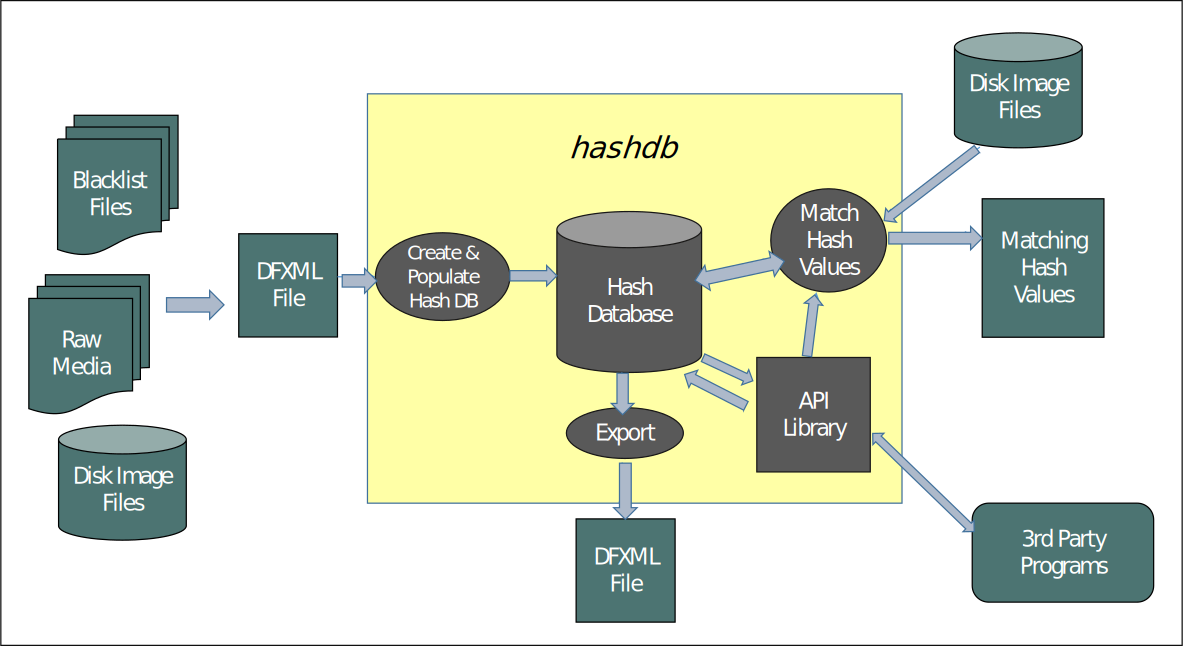
\includegraphics[scale=.45]{drawings/hashdb_system_overview}
	\caption{Overview of the \hdb system}
	\label{fig:overviewFigure}
\end{figure}

\subsection{Blacklist Data}
Blacklist data is the data we scan against to determine whether forensic data
contains probative artifact.
We build a hash database of blacklist data by importing block hashes
from blacklist files, copying from other hash databases,
or importing from other sources using data prepared in JSON format.

\subsection{Forensic Data}
Forensic data is the data we scan to see if it contains artifact matching
that in our hash database.
Note that just having matches is not sufficiently probative.
Some matches are common to many files.
\hdb tracks entropy and data information to automate the process
of eliminating many false positives.
Direct analysis such as that provided by the \sscope tool
may be used to see the exact content at that location.
\sscope is available at \url{https://github.com/NPS-DEEP/NPS-SectorScope/wiki}.

\subsection{Hash Blocks}
\label{HashBlocks}
\hdb works by matching blocks.
\hdb is different from tools that match files because it can find matches
even when part of a file is missing or changed.
\hdb stores and scans for hashes created from contiguous blocks of data.
We call the size of the block hashed the \textit{block size}.
\hdb stores and scans for hashes aligned along sector boundaries.
We call this alignment the \textit{sector size}.
Although larger values take up more space, we have found that the smallest
granularity used by file systems and storage devices is 512 bytes,
so this is the default value for both.

\subsection{Building a \hdb Database}
There are several ways to populate a database:

\begin{itemize}
\item Using the \hdb \verb+import+ command.
\item Importing from correctly formatted JSON data.
\item Importing from another database.
\item Using the \bulk \hdb scanner import function.
\item Using the \hdb library through the Python or C++ interface.
\end{itemize}

A database may contain blacklist hashes from multiple source domains,
where a domain is called a \textit{repository}.
Also, multiple source files can actually be the same source.
To manage this, \hdb tracks sources by source hash,
and a source hash can be referred to by multiple filenames and repository names.

\subsection{Scanning}
There are multiple ways users can scan for matches in a block hash database:

\begin{itemize}
\item Using one of the \hdb tool scan commands to scan from a media image,
list, stream, or specific hash.
\item Using one of the \hdb API scan interfaces to scan at a particular
level of detail.
\item Using the \bulk \hdb scanner Scan function.
\end{itemize}

\subsection{Contents of a Hash Database}
Each \hdb database is contained in a directory called \textit{$<$databasename$>$.hdb} and contains a number of files. These files are:
\begin{verbatim}
lmdb_hash_data_store/data.mdb
lmdb_hash_data_store/lock.mdb
lmdb_hash_store/data.mdb
lmdb_hash_store/lock.mdb
lmdb_source_data_store/data.mdb
lmdb_source_data_store/lock.mdb
lmdb_source_id_store/data.mdb
lmdb_source_id_store/lock.mdb
lmdb_source_name_store/data.mdb
lmdb_source_name_store/lock.mdb
log.txt
settings.json
\end{verbatim}

These files include several data store directories and files, a settings file, and a log file.
Each is described briefly:

\begin{itemize}
\item Data store files \\
The data store files encode all the block hashes, source files, and related information that are in the database.


\item \texttt{log.txt} \\
Every time a command is run that changes the content of the database, this file is replaced with a log of the run.
The log includes the command name, information about \hdb including the command typed and how \hdb was compiled, information about the operating system \hdb was just run on, timestamps indicating how much time the command took, and the specific \hdb changes applied, described in more detail in \textbf{\autoref{Running}}.
\item \texttt{settings.json} \\
This file contains the settings requested by the user when the block hash database was created, see \hdb settings and Bloom filter settings options.
This file also contains internal \hdb settings version used to help \hdb identify whether a database is compatible with this version of \hdb.
\end{itemize}




\subsection{Using the Hash Databases}
\label{usingSection}
\hdb provides the capability for users to scan the database for matching hash blocks. Users can also query for hash source information and information about the hash database itself. \hdb provides an API to access the import and scan capabilities.  The import capability allows third party tools to create a new database at a specified directory, import an array of hashes with source information and write changes to the \texttt{log.xml} file. The scan capability provided by the API allows third party tools to open an existing database and perform a scan. Most importantly, the \bulk \textit{hashdb} scanner uses the \hdb API to provide users with the capability to create databases from disk images or scan digital media and find matching hash blocks within the data \bulk is processing. In later sections, this manual describes the methods for using \bulk together with the \hdb tool. 

\subsection{\bulk}
\bulk is an open source digital forensics tool that extracts features such as email addresses, credit card numbers, URLs and other types of information from digital evidence files. It operates on disk images, files or a directory of files and extracts useful information without parsing the file system or file system structures.  For more information on how to use \bulk for a wide variety of applications, refer to the separate publication \textit{The \bulk Users Manual} available at \url{http://digitalcorpora.org/downloads/bulk_extractor/BEUsersManual.pdf} \cite{beusersguide}.\\

\bulk has multiple scanners that extract features. One particular scanner, the \textit{hashdb} scanner links the full set of \bulk capabilities directly to the \hdb tool. The \textit{hashdb} scanner uses the \hdb API to create and import data into hash databases  directly from the data processed by \bulk. The scanner also can be run with a hash database as input (again using the \hdb API) will scan the data processed by \bulk for matching hash values.\\


\section{Installation Guide}
\hdb is a command line tool that can be run on Linux, MacOS or Windows systems. Here we describe the installation procedures for those systems.
Steps include how to install the required dependencies as well as download \hdb and compile the release or run the executable. 
\label{Installation}

\subsection{Installing on Linux or Mac}

Before compiling \hdb for your platform, you may need to install other packages on your system which \hdb requires to compile cleanly and with a full set of capabilities.\\

\textbf{Dependencies for Linux}\\
The following commands should add the appropriate packages:
\begin{Verbatim}[commandchars=\\\{\}]
\verbbf{sudo yum update}
\verbbf{sudo yum groupinstall development-tools}
\verbbf{sudo yum install gcc-c++}
\verbbf{sudo yum install libxml2-devel openssl-devel tre-devel boost-devel}
\end{Verbatim}

\textbf{Dependencies for Mac Systems}\\
Mac users must first install Apple's Xcode development system. Other components should be downloaded using the MacPorts system. If you do not have MacPorts, go to the App store and download and install it. It is free. Once it is installed, try:
\begin{Verbatim}[commandchars=\\\{\}]
\verbbf{sudo port install autoconf automake libxml2} 
\end{Verbatim}

\textbf{Download and Install \hdb}\\
Next, download the latest version of \hdb. The software can be downloaded from \url{http://digitalcorpora.org/downloads/hashdb/}. The file to download is \texttt{hashdb-x.y.z.tar.gz} where x.y.z is the latest version. As of publication of this manual, the latest version of \hdb is 1.1.1.\\


After downloading the file, un-tar it by either right-clicking on the file and choosing ``extract to...' or typing the following at the command line:
\begin{Verbatim}[commandchars=\\\{\}]
\verbbf{tar -xvf hashdb-x.y.z.tar.gz}
\end{Verbatim}

Then, in the newly created \textit{hashdb-x.y.z} directory, run the following commands to install \hdb in \textit{/usr/local/bin} (by default):

\begin{Verbatim}[commandchars=\\\{\}]
\verbbf{./configure}
\verbbf{make}
\verbbf{sudo make install}
\end{Verbatim}
\hdb is now installed on your system and can be run from the command line. \\

Note: sudo is not required. If you do not wish to use sudo,  build and install \hdb and \bulk in your own space at ``\$HOME/local'' using the following commands:
\begin{Verbatim}[commandchars=\\\{\}]
\verbbf{./configure --prefix=$HOME/local/ --exec-prefix=$HOME/local CPPFLAGS=-}
\textbf{                                 I$HOME/local/include/ LDFLAGS=-L$HOME/local/lib/}
\verbbf{make}
\verbbf{make install}
\end{Verbatim}

\subsection{Installing on Windows}
\label{InstallingOnWindows}
Windows users should download the Windows Installer for \hdb. The file to download is located at \url{http://digitalcorpora.org/downloads/hashdb} and is called \texttt{hashdb-x.y.} \texttt{z-windowsinstaller.exe} where x.y.z is the latest version number (1.1.1 as of publication of this manual).\\

You should close all Command windows before running the installation executable. Windows will not be able to find the \hdb tools in a Command window if any are open during the installation process. If you do not do this before installation, simply close all Command windows after installation. When you re-open, Windows should be able to find \hdb.\\


 Next run the \texttt{hashdb-x.y.z-windowsinstaller.exe} file. This will automatically install \hdb on your machine. Some Windows safeguards may try to prevent you from running it. Figure \ref{fig:windowsWarning} shows the message Windows 8 displays when trying to run the installer. To run anyway, click on ``More info'' and then select ``Run Anyway.'' \\
\begin{figure}
	\center
	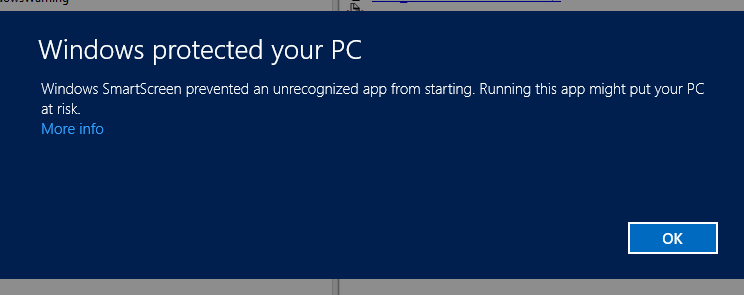
\includegraphics[scale=.5]{windowsWarning.png}
	\caption{Windows 8 warning when trying to run the installer. Select ``More Info'' and then ``Run Anyway.''}
	\label{fig:windowsWarning}
\end{figure}

When the installer file is executed, the installation will begin and show a dialog like the one shown in Figure \ref{fig:windowsInstaller}.  Users should select the 64-bit configuration to install \hdb and select \verb+Add to path+ to add hashdb to \verb+PATH+. \hdb is now installed on your system can be run from the command line.\\

\begin{figure}
	\center
	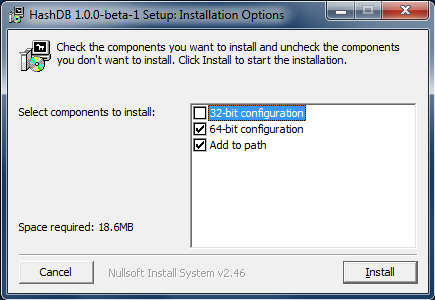
\includegraphics[scale=.8]{WindowsInstaller.png}
	\caption{Dialog appears when the user executes the Windows Installer. Select the default configuration.}
	\label{fig:windowsInstaller}
\end{figure}

\subsection{Installing Other Related Tools}

\subsubsection{\bulk}
The \bulk \hdb scanner provides the capability to import block hashes into a new hash database and to scan for hashes against an existing hash database.
\hdb requires a newer build of \bulk.
Please see the \hdb Wiki page at \url{https://github.com/NPS-DEEP/hashdb/wiki}
for information on obtaining a compatible version of \bulk.

\subsubsection{\sscope}
The \sscope tool provides a GUI for analyzing data associated with hash matches found by \hdb.
\sscope also provides an Autopsy plug-in module for running \hdb and \sscope from within the Autopsy framework.
Please see the \sscope Wiki page at \url{https://github.com/NPS-DEEP/NPS-SectorScope/wiki}
for information on downloading and using \sscope.

\section {Running the \hdb Tool}
\label{Running}
The core capabilities provided by \hdb involve creating and maintaining a database of hash values and scanning media for those hash values. To perform those tasks, \hdb users need to start by building a database (if an existing database is not available for use).
Users then import hashes using \hdb commands, the \hdb \bulk scanner, or the \hdb API, and then possibly merge or subtract hashes to obtain the desired set of hashes to scan against.
Users then scan for hashes that match.
Additional commands are provided to support statistical analysis, performance tuning and performance analysis.\\

This section describes \hdb commands, along with examples, for performing these tasks.
For more examples of command usage, please see \textbf{\autoref{UseCases}}.
For a \hdb quick reference summary, please see \textbf{\autoref{QuickReference}}
or \url{http://digitalcorpora.org/downloads/hashdb/hashdb_quick_reference.pdf}.

\subsection{Creating a Hash Database}
A hash database must be created before hashes can be added to it.
The command to create a hash database is shown in Table \ref{tab:createDatabase}.
\begin{table}[!ht]
\centering
\caption{Command for Creating Hash Databases}
\label{tab:createDatabase}
\begin{tabular}{|p{2.5 cm}|p{7 cm}|p{4 cm}|}
\hline \hline
\textbf{Command} & \textbf{Usage} & \textbf{Description} \\
\hline
\textbf{create} & \verb+create [-b <block size>]+ \verb+[-b <sector size>]+ \verb+[-m <max ID offset pairs>]+ \verb+[-t <hash prefix bits:hash+ \verb+suffix bytes>]+ \verb+<hashdb.hdb>+ & Creates a new hash database with the given configuration settings.\\
\hline
\end{tabular}
\end{table}

Table \ref{tab:hashDBSettings} shows the configurable database settings.\\

\begin{table}[!ht]
\centering
\caption{Settings for New Databases}
\label{tab:hashDBSettings}
\begin{tabular}{|p{1.5 cm}|p{8 cm}|p{4 cm}|}
\hline \hline
\textbf{Option} & \textbf{Verbose Option} & \textbf{Specification} \\
\hline
\textbf{\texttt{-b}} & \verb+--block_size=+\textit{block\_size} & Specifies the block size in bytes used to generate the hashes that will be stored in the database. Default is 512 bytes.  \\
\hline
\textbf{\texttt{-s}} & \verb+--sector_size=+\textit{sector\_size} & Specifies the sector size in bytes used to calculate hashes along. Default is 512 bytes.  \\
\hline
\textbf{\texttt{-m}} & \verb+--max_source_offset_pairs=+\textit{max source offset pairs} & Specifies the maximum number of source, source offset pairs allowed. 0 value indicates there is no limit. Default is 0.\\
\hline
\textbf{\texttt{-t}} & \verb+--tuning=+\textit{prefix bits:suffix bytes} & Specifies the number of prefix bits and suffix bytes to use for compacting the database.\\
\hline
\end{tabular}
\end{table}



\textbf{Block size}\\
The size of data blocks the database expects to store. Block hashes are calculated from data of this size. The default is 512.\\

\textbf{Sector size}\\
The resolution of sectors that may reside on media. The operating system and/or storage device will align data on sector boundaries. Block hashes are calculated on aligned sector boundaries. The default is 512.\\

\textbf{Max ID offset pairs}\\
The maximum number of source, offset pairs to store for a given hash, default 100,000. Each pair identifies a location in a source where this hash is located. If source information is not interesting when there are many sources, offset pairs associated with a hash, use a low value to prevent storing extra entries.\\

\textbf{Hash prefix bits}\\
The number of bits of the hash prefix to use as the key in the store. The idea is to select a value given the size of the database so that the average number of hashes with this prefix is slightly greater than 0, for example 20. For example if you expect 5 billion hashes, you might select 28 because $5/2^{28}=18.6$, which is near 20.\\

\textbf{hash suffix bytes}\\
The number of bytes of the hash suffix to store in the set of values of hash suffixes for this hash key. The idea is to store as few bytes as possible while minimizing false positives. For example if you expect 5 billion hashes, you might select 28 prefix bits and 3 suffix bytes because $5 / 2^{((28) + 8*(3))} = 5 / 2^{52} = 0.00011\%$ false positive rate, about 1 in 1 million.\\

\textbf{Example}\\
To create an (empty) hash database named \textbf{\texttt{mock\_video.hdb}}, type the following command:
\begin{Verbatim}[commandchars=\\\{\}]
\verbbf{hashdb create mock_video.hdb}
\end{Verbatim}
The above command will create a database with all of the default hash database settings. Most users will not need to change these settings.
Users can specify either the option and value or the verbose option value for each parameter along with the create command, as in:\\
\begin{Verbatim}[commandchars=\\\{\}]
\verbbf{hashdb create --max\_source\_offset\_pairs=20 mock_video.hdb}
\verbbf{hashdb create -m 20 mock_video.hdb}
\end{Verbatim}
The above two commands produce identical results, creating the database \texttt{mock\_video.hdb} that will accept a maximum of 20 source, offset pairs per hash.\\

\subsection{Importing and Exporting}
Hash databases may be imported to in several ways, and may be exported in JSON format.
Commands to import and export hashes are shown in Table \ref{tab:importExport}.\\
\begin{table}[!ht]
\centering
\caption{Commands for Importing into and Exporting Hash Databases}
\label{tab:importExport}
\begin{tabular}{|p{2.5 cm}|p{7 cm}|p{4 cm}|}
\hline \hline
\textbf{Command} & \textbf{Usage} & \textbf{Description} \\
\hline
\textbf{import\_dir} & \verb+import_dir [-r <repository name>]+ \verb+[-w <whitelist.hdb>]+ \verb+<hashdb.hdb>+ \verb+<import directory>+& Imports hashes from files under the import directory.\\
\hline
\textbf{import\_tab} & \verb+import_tab [-r <repository name>]+ \verb+<hashdb.hdb>+ \verb+<tab.txt>+& Imports values from the tab-delimited file into the hash database.\\
\hline
\textbf{import} & \verb+import <hashdb.hdb>+ \verb+<hashdb.json>+& Imports values from the JSON file into the hash database.\\
\hline
\textbf{export} & \verb+export <hashdb.hdb>+ \verb+<hashdb.json>+& Exports the hash database to the JSON file\\
\hline
\end{tabular}
\end{table}
Note that there are other ways to populate a database besides these listed here, including using other hash databases (discussed in \textbf{\autoref{updateSection}}),
by using the \bulk \hdb scanner (discussed in \textbf{\autoref{bulkextractorSection}}),
and through the use of the import capability provided by the \hdb library API (discussed in \textbf{\autoref{APISection}}).\\

The tab-delimited import file consists of hash lines separated by carriage returns, where each line consists of a filename followed by a tab followed by the file hash followed by a sector index that starts at 1.  Comment lines are allowed by starting them with the \texttt{\#} character.
An example tab-delimited file is shown in Listing \ref{importTabFile}.

\lstset{style=customfile}
\begin{lstlisting}[float, caption={Example content of a tab-delimited import file}, label=importTabFile]
# tab-delimited import file
file1	3b6b477d391f73f67c1c01e2141dbb17	1
file1	89a170b6b9a948d21d1d6ee1e7cdc467	2
file1	f58a09656658c6b41e244b4a6091592c	3
\end{lstlisting}


To import block hashes from a directory of blacklist sources, type the following command:
\begin{Verbatim}[commandchars=\\\{\}]
\verbbf{hashdb import_dir -r mock_video_repository mock_video.hdb mock_video_dir}
\end{Verbatim}
In the above command the option \textbf{-r} is used along with the repository name \texttt{mock\_video\_repository} to indicate the repository source of the block hashes being imported into the database. The repository name is used to keep track of the sources of hashes. Hash blocks contained in one database often originate from many different sources and the fileme may be the same. For example, if we add two separate but similar databases with partial overlap to a database, this will result in some duplicate hashes from multiple sources with the same filename. The repository name can be used with those duplicates to allow users to track all hashes back to their original sources. By default, the repository name used is the text \texttt{repository\_} with the filename of the file being imported from appended after it.\\

The \textbf{import} command in the above example imports block hashes from files in the \texttt{mock\_video\_dir} directory into the database \texttt{mock\_video.hdb}. \hdb prints the following to the command line to indicate that the hashes have been inserted into the database successfully: 

\begingroup
\footnotesize
\begin{Verbatim}[fontfamily=courier]
zzz replace with correct data
#    hashes inserted: 2595
\end{Verbatim}
\endgroup
The database \texttt{\textbf{mock\_video.hdb}} now contains these block hashes.

The file \texttt{log.txt} shows that a set of hash blocks have just been inserted. Listing \ref{logexcerpt} shows the excerpt of the log file that tracks this statistic.
\lstset{style=customfile}
\begin{lstlisting}[float, caption=Excerpt of the \texttt{log.xml} indicating hash blocks were inserted, label=logexcerpt]
zzz replace with correct data
...   
   <repository_name>mock_video_repository</repository_name>
    <timestamp name='begin import' delta='0.024016' total='0.024016'/>
    <timestamp name='end import' delta='0.015009' total='0.039025'/>
    <hashdb_changes>
      <hashes_inserted>2595</hashes_inserted>      
    </hashdb_changes>
...
\end{lstlisting}
Users may prefer to run statistical commands such as this to get information about the contents of the database (and confirm that values were inserted):
\begin{Verbatim}[commandchars=\\\{\}]
\verbbf{hashdb size mock_video.hdb}
\end{Verbatim}

\subsection{Database Manipulation}
\label{DatabaseManipulation}
Databases may need to be merged together or common hash values may need to be subtracted out in order for them to be more suitable for scanning against.
Commands that manipulate hash databases are outlined in Table \ref{tab:databaseManipulation}.
Destination databases are created if they do not exist yet.

\begin{table}[!ht]
\centering
\caption{Commands to Manipulate Hash Databases}
\label{tab:databaseManipulation}
\begin{tabular}{|p{3.5 cm}|p{6 cm}|p{4 cm}|}
\hline \hline
\textbf{Command} & \textbf{Usage} & \textbf{Description} \\
\hline
\textbf{add} & \verb+add <source db>+ \verb+<destination db>+ & Copies all of the hashes from \textit{source db} to \textit{destination db}\\
\hline
\textbf{add\_multiple} &  \verb+add_multiple <source db1>+ \verb+<source db2> <destination db>+ & Performs the union of \textit{source db1} and \textit{source db2} and copies all of the hash values from the union into \textit{destination db}\\
\hline
\textbf{add\_repository} & \verb+add_repository <source db1>+ \verb+<destination db2>+ \verb+<repository namedb>+ & Adds \textit{source db1} to \textit{destination db2} but only when the repository name matches\\
\hline
\textbf{intersect} & \verb+intersect <source db1>+ \verb+<source db2> <destination db>+ &   Copies hash values common to both \textit{source db1} and \textit{source db2} into \textit{destination db} where sources match\\
\hline
\textbf{intersect\_hash} & \verb+intersect_hash <source db1>+ \verb+<source db2> <destination db>+ &   Copies hash values common to both \textit{source db1} and \textit{source db2} into \textit{destination db} even when source repository name and filename do not match\\
\hline
\textbf{subtract} & \verb+subtract <source db1>+ \verb+<source db2> <destination db>+&   Copies hash values found in \textit{source db1} but not in \textit{source db2} into \textit{destination db} where sources match\\
\hline
\textbf{subtract\_hash} & \verb+subtract <source db1>+ \verb+<source db2> <destination db>+&   Copies hash values found in \textit{source db1} but not in \textit{source db2} into \textit{destination db} even when source repository name and filename do not match\\
\hline
\textbf{subtract \_repository} & \verb+subtract_repository+ \verb+<source db1>+ \verb+<destination db2>+ \verb+<repository namedb>+ & Adds \textit{source db1} to \textit{destination db2} unless the repository name matches\\
\hline
\textbf{deduplicate} & \verb+deduplicate <source db>+ \verb+<destination db>+ &   Copies all non-duplicate hash values from \textit{source db} into \textit{destination db}\\
\hline
\end{tabular}
\end{table}

\subsubsection{Tracking Changes in Hash Databases}
Statistics about hash database changes are reported on the console and to the log file and history file inside the hash database.
These statistics show the number of hashes inserted into a database as a result of a command, and also show the number of hashes not removed because specific conditions were not met.
These statistics are shown in Table \ref{tab:changeStatistics}.
\begin{table}[!ht]

\centering
\caption{Database Changes Resulting from Commands that Manipulate Hash Databases}
\label{tab:changeStatistics}
\begin{tabular}{|p{5 cm}|p{8.8 cm}|}
\hline \hline
\textbf{Statistic} & \textbf{Meaning} \\
\hline
\verb+hashes_inserted+ &  Number of hashes inserted.\\
\hline
\verb+hashes_not_inserted_+ \verb+invalid_byte_alignment+ &  Number of hashes not inserted because the file offset was not byte aligned.
If the database expects a byte alignment of 512 and the \hdb user
tries to add a hash at byte 80, \hdb will detect that 80 does not fall on
a 512 byte boundary (80 mod 512 $\ne$ 0).\\
\hline
\verb+hashes_not_inserted_+ \verb+exceeds_max_duplicates+ & Number of hashes not inserted because they exceed the max duplicates value. For example, user sets max duplicates with \texttt{-m 20} and the run attempts to import 30 hashdigests calculated from 30 NULL blocks of input, so we see 20 max duplicates.\\
\hline
\verb+hashes_not_inserted_+ \verb+duplicate_element+ & Number of hashes not inserted because they are duplicate elements. The user attempts to import a hash where the hash value, repository name, filename, and its file offset
are all the same.\\
\hline
% note: manipulation commands do not remove hashes, they copy them.
%\verb+hashes_removed+ & Number of hashes removed.\\
%\hline
%\verb+hashes_not_removed_+ \verb+invalid_byte_alignment+ &  Number of hashes not removed because the file offset was not byte aligned.\\
%\hline
%\verb+hashes_not_removed_+ \verb+no_hash+ &  Number of hashes not removed because the hash blocks requested for removal did not exist in the database.\\
%\hline
%\verb+hashes_not_removed_+ \verb+no_element+ &  Number of hashes not removed because the hashes, specifically identified by 
%hash value, repository name, filename, and its file offset do not exist in the database, indicating a possible mistake in database management.\\
%\hline
\end{tabular}
\end{table}

\subsection{Scan Services}
\label{ScanServices}
\hdb can be used to determine if a file, directory or disk image has content that matches previously identified content. This capability can be used, for example, to determine if a set of files contains a specific file excerpt or if a media image contains a video fragment. Forensic investigators can use this feature to search for blacklisted content. To scan media for hash values, run using the \bulk \textit{hashdb} scanner on a media image file and provide a hash database created by \hdb as input.
Scan services are shown in Table \ref{tab:scanServices}. \\

\begin{table}[!ht]
\centering
\caption{Commands that Provide Scan Services}
\label{tab:scanServices}
\begin{tabular}{|p{3.5 cm}|p{6 cm}|p{4 cm}|}
\hline \hline
\textbf{Command} & \textbf{Usage} & \textbf{Description} \\
\hline
\textbf{scan} & \verb+scan <path>+ \verb+<DFXML file>+ & Scans the hashdb for hashes that match hashes in the DFXML file and prints out matches\\
\hline
\textbf{scan\_hash} & \verb+scan_hash <path>+ \verb+<hash value>+ & Scans the hashdb for the specified hash value and prints out whether it matches\\
\hline
\textbf{scan\_expanded} & \verb+scan_expanded [-m <number>]+ \verb+<hashdb> <DFXML file>+ & Scans the hashdb for hashes that match hashes in the DFXML file and unless more than max, prints out the repository name, filename, and file offset for each hash that matches\\
\hline
\textbf{scan\_expanded\_} \textbf{hash} & \verb+scan_expanded_hash+ \verb+[-m <number>] <hashdb>+ \verb+<hash value>+ & Scans the hashdb for the specified hash value and unless more than max, prints out the repository name, filename, and file offset for each hash that matches\\
\hline
\end{tabular}
\end{table}

First, identify the media that you would like to scan. For this example, we download and use video file \texttt{mock\_video\_redacted\_image} available at \url{http://digitalcorpora.org/downloads/hashdb/demo}.\\ 

Second, identify the existing hash database that will be used to search for hash value matches. We'll use the database \texttt{\textbf{mock\_video.hdb}} that we created in the previous section. That database contains all of the block hash values from a media image. \\

Finally, run \bulk from the command line and send the required parameters to the \textit{hashdb} scanner using the \textbf{-S} option. Run the following command: 
\begin{Verbatim}[commandchars=\\\{\}]
\verbbf{bulk_extractor -e hashdb -o outdir -S hashdb_mode=scan \\}
\textbf{    -S hashdb_scan_path_or_socket=mock_video.hdb mock_video_redacted_image}
\end{Verbatim}
This command tells \bulk to enable the \textit{hashdb} scanner and to run it in ``scan'' mode to try to match the values found in the local database \texttt{\textbf{mock\_video.hdb}}. Note: other run options using \bulk are discussed further in \textbf{\autoref{bulkextractorSection}}.\\

Listing \ref{bulkHashScan} shows the output printed to the command line as a result of the above \bulk \hdb scan command. \\

\lstset{style=customfile}
\begin{lstlisting}[float, caption=Output from \bulk \hdb scan, label=bulkHashScan]
bulk_extractor version: 1.4.1
Input file: mock_video_redacted_image
Output directory: outdir1
Disk Size: 12596738
Threads: 4
All data are read; waiting for threads to finish...
Time elapsed waiting for 1 thread to finish:
     (timeout in 60 min .)
Time elapsed waiting for 1 thread to finish:
    6 sec (timeout in 59 min 54 sec.)
Thread 0: Processing 0

All Threads Finished!
Producer time spent waiting: 0 sec.
Average consumer time spent waiting: 4.69167 sec.
Phase 2. Shutting down scanners
Phase 3. Creating Histograms
   ccn histogram...   ccn_track2 histogram...   domain histogram...
   email histogram...   ether histogram...   find histogram...
   ip histogram...   telephone histogram...   url histogram...
   url microsoft-live...   url services...   url facebook-address...
   url facebook-id...   url searches...
Elapsed time: 6.33812 sec.
Total MB processed: 125
Overall performance: 1.98746 MBytes/sec (0.496864 MBytes/sec/thread)
Total email features found: 0
\end{lstlisting}

All hash block matches discovered in the hash database are printed to the \bulk output file \texttt{identified\_blocks.txt}. Listing \ref{identifiedBlocks} shows the contents of that file after the \bulk run. Each line of the file corresponds to one hash block from the input data provided that was matched in the database. The number at the beginning of the line is the Forensic Path.\\


The second column of the \texttt{identified\_blocks.txt} file shows the actual block hash value. The final column is the number of times this block hash value has been added to the hash database. It is a count of hash duplicates. Hash duplicates occur when the hash value is the same but any part of the source information including repository name, filename or offset, is unique. In this case, each hash values shown has only been added to the database once.\\

\lstset{style=customfile}
\begin{lstlisting}[float, caption={The \texttt{identified\_blocks.txt} file produced by \bulk's \textit{hashdb} scanner. First column is the forensic path, second is the hash value, and third is the number of times the hash value occurs in the database}, label=identifiedBlocks]
# BANNER FILE NOT PROVIDED (-b option)
# BULK_EXTRACTOR-Version: 1.5.5-dev ($Rev: 10844 $)
# Feature-Recorder: identified_blocks
# Filename: /home/bdallen/demo8/demo_video_redacted_image
# Feature-File-Version: 1.1
12452352	3b6b477d391f73f67c1c01e2141dbb17	{"count":1}
12456448	89a170b6b9a948d21d1d6ee1e7cdc467	{"count":1}
12460544	f58a09656658c6b41e244b4a6091592c	{"count":1}
12464640	1d0abbddf1344ac751d17604bdd9ebe8	{"count":1}
12468736	16d75027533b0a5ab900089a244384a0	{"count":1}
12472832	97068927ff7ca0c4d27ac527474065bc	{"count":1}
12476928	80a403ea48854676501a02e390a69699	{"count":1}
12481024	7de953ea563c4df1f8369d8dd2cfb4d9	{"count":1}
12485120	1b803bd6e014d1855e6f8413041c2b07	{"count":1}
12489216	cf49adf3285b983d9f8d60497290bfd2	{"count":1}
12493312	4cc415709e205ac0ef5b5dcfb77936b6	{"count":1}
12497408	0c5c611edc8dfd34f85c6cbf88702e51	{"count":1}
12501504	4a93e65fb187d71c2b8b5697f1460e3d	{"count":1}
12505600	a667f79e6446222092257af1780f6a9f	{"count":1}
12509696	aec94ab99f591f507b3c27424a0b52c5	{"count":1}
12513792	c6361fe0eb4f7b13bac6529e1cdd8ea4	{"count":1}
\end{lstlisting}

\begin{lstlisting}[float, caption={Two lines from the \texttt{identified\_sources.txt} file produced by post-processing the \texttt{identified\_blocks.txt} file. The third column is replaced with expaned information}, label=identifiedSourceLine]
12452352	3b6b477d391f73f67c1c01e2141dbb17	[{"count":1},{"sou
rce_list_id":2844319735, "sources":[{"source_id":1,"file_offset":10485760,
"repository_name":"temp1","filename":"\/home\/bdallen\/demo8\/demo_video.m
p4","filesize":10630146,"file_hashdigest":"a003483521c181d26e66dc09740e939
d"}]}]
12456448	89a170b6b9a948d21d1d6ee1e7cdc467	[{"count":1},{"sou
rce_list_id":2844319735, "sources":[{"source_id":1,"file_offset":10489856}
]}]
\end{lstlisting}

Users may be put off by the quantity of matches incurred by low-entropy data in their databases such as blocks of zeros or metadata header blocks from files that are otherwise unique. Database manipulation commands,
\textbf{\autoref{DatabaseManipulation}}, can mitigate this, for example:
\begin{itemize}
\item Use the ``subtract'' command to remove known whitelist data created from sources such as ``brand new'' operating system images and the NSRL.
\item Alternatively, use the ``deduplicate'' command to copy all hash values that have been imported exactly once.
\end{itemize}
These commands are provided to manage false positives.

\subsection{Statistics}
Various statistics are available about a given hash database including the size of a database, where its hashes were sourced from, a histogram of its hashes, and more.
Table \ref{tab:statistics} describes available statistics.\\

\begin{table}[!ht]
\centering
\caption{Commands that provide Statistics about Hash Databases}
\label{tab:statistics}
\begin{tabular}{|p{3.5 cm}|p{6 cm}|p{4 cm}|}
\hline \hline
\textbf{Command} & \textbf{Usage} & \textbf{Description} \\
\hline
\textbf{size} & \verb+size <hashdb>+ & Prints out size information relating to the database\\
\hline
\textbf{sources} & \verb+sources <hashdb>+ & Provides a top-level view of the repository names and filenames in the database. It prints out all repositories and files that have contributed to this database\\
\hline
\textbf{histogram} & \verb+histogram <hashdb>+ &  Prints a hash distribution for the hashes in the \textit{hashdb}\\
\hline
\textbf{duplicates} & \verb+duplicates <hashdb> <number>+ &  Prints out hashes in the database that are sourced the given number of times\\
\hline
\textbf{hash\_table} & \verb+hash_table <hashdb> <source_id>+ &  Prints hashes associated with the specified source index in a format compatible with \texttt{identified\_blocks.txt} files\\
\hline
\textbf{expand\_identified} \textbf{\_blocks} & \verb+expand_identified_blocks+ \verb+[-m <number>] <hashdb>+ \verb+<identified_blocks.txt>+ & Prints expanded source information from the \textit{hashdb} unless more than max, default 200, of each hash in the \texttt{identified\_blocks.txt} input file\\
\hline
\textbf{explain\_identified} \textbf{\_blocks} & \verb+expand_identified_blocks+ \verb+[-m <number>] <hashdb>+ \verb+<identified_blocks.txt>+ & Prints out hash and source tables for sources with hashes observed no more than the maximum number of times, default max 20, for each hash feature in the \texttt{identified\_blocks.txt} input file\\
\hline
\end{tabular}
\end{table}

To identify the source information associated with the hash values found in \texttt{identified\_blocks.txt}, type the following command using the hash database and \texttt{identified\_blocks.txt} file as input (command should be run from the same directory in which you ran \bulk):
\begin{Verbatim}[commandchars=\\\{\}]
\verbbf{hashdb expand_identified_blocks mock_video.hdb outdir/identified_blocks.txt} 
\textbf{  > identified_sources.txt}
\end{Verbatim}
The above command pipes the output directly into the file \texttt{identified\_sources.txt}. Each line of the file will provide the source information for one of the identified hash blocks. An example line from this file is shown in Listing \ref{identifiedSourceLine},
which shows that the block at Forensic path 12464640 matches the block 10498048 bytes into the \texttt{mock\_video.mp4} files in the hash database, indicating a positive match.\\

A table of more relevant hashes and source information may be generated using the \verb+explain_identified_blocks+ command.
To generate these tables for \texttt{identified\_blocks.txt}, type the following command using the hash database and \texttt{identified\_blocks.txt} file as input (command should be run from the same directory in which you ran \bulk):
\begin{Verbatim}[commandchars=\\\{\}]
\verbbf{hashdb explain_identified_blocks mock_video.hdb outdir/identified_blocks.txt} 
\textbf{  > explained_hashes_and_sources.txt}
\end{Verbatim}
The above command pipes the output directly into the file \texttt{explain\_hashes\_and\_sources.txt}.
The output of this command is shown in Listing \ref{explainHashesAndSources}.
The first table in file \texttt{explain\_hashes\_and\_sources.txt}
shows block hashes, their source ID, and the offset into the file where they were sourced from.
The second table in the file shows sources, in this case, just one source corresponding to source ID 1.
Each line of source information describes
the repository name, filename, file size, and file hash for a given source ID.\\

\begin{lstlisting}[float, caption={The \texttt{identified\_hashes\_and\_sources.txt} file produced by post-processing the \texttt{identified\_blocks.txt} file using the \texttt{explain\_identified\_blocks} command}, label=explainHashesAndSources]
 hashdb-Version: 2.0.0
# explain_identified_blocks-command-Version: 3
# command_line: hashdb explain_identified_blocks temp1.hdb temp2/identifie
d_blocks.txt
# hashes
["0c5c611edc8dfd34f85c6cbf88702e51",{"count":1},[{"source_id":1,"file_offs
et":10530816}]]
["16d75027533b0a5ab900089a244384a0",{"count":1},[{"source_id":1,"file_offs
et":10502144}]]
["1b803bd6e014d1855e6f8413041c2b07",{"count":1},[{"source_id":1,"file_offs
et":10518528}]]
["1d0abbddf1344ac751d17604bdd9ebe8",{"count":1},[{"source_id":1,"file_offs
et":10498048}]]
["3b6b477d391f73f67c1c01e2141dbb17",{"count":1},[{"source_id":1,"file_offs
et":10485760}]]
["4a93e65fb187d71c2b8b5697f1460e3d",{"count":1},[{"source_id":1,"file_offs
et":10534912}]]
["4cc415709e205ac0ef5b5dcfb77936b6",{"count":1},[{"source_id":1,"file_offs
et":10526720}]]
["7de953ea563c4df1f8369d8dd2cfb4d9",{"count":1},[{"source_id":1,"file_offs
et":10514432}]]
["80a403ea48854676501a02e390a69699",{"count":1},[{"source_id":1,"file_offs
et":10510336}]]
["89a170b6b9a948d21d1d6ee1e7cdc467",{"count":1},[{"source_id":1,"file_offs
et":10489856}]]
["97068927ff7ca0c4d27ac527474065bc",{"count":1},[{"source_id":1,"file_offs
et":10506240}]]
["a667f79e6446222092257af1780f6a9f",{"count":1},[{"source_id":1,"file_offs
et":10539008}]]
["aec94ab99f591f507b3c27424a0b52c5",{"count":1},[{"source_id":1,"file_offs
et":10543104}]]
["c6361fe0eb4f7b13bac6529e1cdd8ea4",{"count":1},[{"source_id":1,"file_offs
et":10547200}]]
["cf49adf3285b983d9f8d60497290bfd2",{"count":1},[{"source_id":1,"file_offs
et":10522624}]]
["f58a09656658c6b41e244b4a6091592c",{"count":1},[{"source_id":1,"file_offs
et":10493952}]]
# sources
{"source_id":1,"repository_name":"temp1","filename":"\/home\/bdallen\/demo
8\/demo_video.mp4","filesize":10630146,"file_hashdigest":"a003483521c181d2
6e66dc09740e939d"}
\end{lstlisting}

\subsection{Tuning}
Tuning commands are provided to improve performance,
see Table \ref{tab:tuning}.
For Bloom filter settings, see Table \ref{tab:bloomSettings}.

\begin{table}[!ht]
\centering
\caption{Commands that Tune Hash Databases}
\label{tab:tuning}
\begin{tabular}{|p{3.5 cm}|p{6 cm}|p{4 cm}|}
\hline \hline
\textbf{Command} & \textbf{Usage} & \textbf{Description} \\
\hline
\textbf{rebuild\_bloom} & \verb+rebuild_bloom[--bloom <state>]+ \verb+[--bloom_n <n>]+ \verb+[--bloom_kM <k:M>]+ \verb+<hashdb.hdb>+ & Rebuilds the Bloom filter using the provided settings, see Table \ref{tab:bloomSettings}\\
\hline
\end{tabular}
\end{table}

\subsection{Performance Analysis}
Performance analysis commands for analyzing \hdb performance are available, see Table \ref{tab:analysis}.

\begin{table}[!ht]
\centering
\caption{Commands that Support \hdb Performance Analysis}
\label{tab:analysis}
\begin{tabular}{|p{3.5 cm}|p{6 cm}|p{4 cm}|}
\hline \hline
\textbf{Command} & \textbf{Usage} & \textbf{Description} \\
\hline
\textbf{add\_random} & \verb+add_random+ \verb+-r [<repository name>]+ \verb+<hashdb.hdb> <count>+ & Adds count random hashes to the given database, creating timing data in the \texttt{log.xml} file\\
\hline
\textbf{scan\_random} & \verb+scan_random <hashdb.hdb>+ & Scans the given database, creating timing data in the \texttt{log.xml} file\\
\hline
\end{tabular}
\end{table}

\subsection{Importing and Scanning Using the \bulk \hdb Scanner}
\label{ImportingAndScanning}
The \bulk \hdb scanner may be used to import hashes and to scan for hashes.
Example syntax for this scanner is shown in Table \ref{tab:hashdbScanner}.
Scanner options are shown in Table \ref{tab:hashdb_be_usage}.

\begin{table}[!ht]
\centering
\caption{\bulk \hdb Scanner Commands}
\label{tab:hashdbScanner}
\begin{tabular}{|p{3.5 cm}|p{6 cm}|p{4 cm}|}
\hline \hline
\textbf{Mode} & \textbf{Example} & \textbf{Description} \\
\hline
\textbf{import} & \verb+bulk_extractor -E hashdb+ \verb+-S hashdb_mode=import+ \verb+-o outdir1 my_image1+ & Import hashes from image into outdir1/hashdb.hdb\\
\hline
\textbf{scan} & \verb+bulk_extractor -E hashdb+ \verb+-S hashdb\_mode=scan+ \verb+-S hashdb_scan_path_or_socket+ \verb+=outdir1/hashdb.hdb -o outdir2+ \verb+my_image+ & Scan image for hashes matching hashes in outdir1/hashdb.hdb\\
\hline
\end{tabular}
\end{table}

\begin{table}[!ht]

\centering
\caption{\bulk \hdb Scanner Options}
\label{tab:hashdb_be_usage}
%\begin{tabular}{|p{3.5 cm}|p{6 cm}|p{4 cm}|}
\begin{tabular}{|p{5 cm}|p{2.0 cm}|p{6.5 cm}|}
\hline \hline
\textbf{Option} & \textbf{Default} & \textbf{Specification} \\
\hline
\verb+hashdb_mode+ & \verb+none+ & The mode for the scanner, one of \verb+[none|import|scan]+. For ``none'', the scanner is active but performs no action. For ``import'', the scanner imports block hashes. For ``scan'', the scanner scans for matching block hashes.\\
\hline
\verb+hashdb_block_size+ &4096 & Block size, in bytes, used to generate hashes.\\
\hline
\verb+hashdb_ignore_empty_blocks+ & \verb+YES+ &Selects to ignore empty blocks,  one of \verb+[YES|NO]+.\\
\hline
\verb+hashdb_scan_path_or_socket+ & & The file path to a hash database or socket to a hashdb server to scan against.  Valid only in scan mode. No default provided. Value must be specified if in scan mode.  Currently, socket server mode is unavailable.\\
\hline
\verb+hashdb_scan_sector_size+ & 512 &Selects the scan sector size.  Scans along sector boundaries.  Valid only in scan mode.\\
\hline
\verb+hashdb_scan_max_features+ & 0 &The maximum number of feature lines to record or 0 for no limit.  Valid only in scan mode.\\
\hline
\verb+hashdb_import_sector_size+ & 4096 & Selects the import sector size.  Imports along sector boundaries.  Valid only in import mode.\\
\hline
\verb+hashdb_import_repository_+ \verb+name+ & \verb+default_+ \verb+repository+ &Selects the repository name to attribute the import to.  Valid only in import mode.\\
\hline
\verb+hashdb_import_max_+ \verb+duplicates+ & 0 &The maximum number of duplicates to import for a given hash value.  Valid only in import mode. Use default of 0 for no limit.\\
\hline
\end{tabular}
\end{table}

\section{Use Cases for \hdb}
\label{UseCases}
There are many different ways to utilize the functionality provided by the \hdb tool. In this section, we highlight some of the most common uses of the system.

\subsection{Querying for Source or Database Information}
 Users can scan a hash database directly using various querying commands. Those commands are outlined in Table \ref{tab:scanServices}.  The ``scan'' command allows users to search for hash blocks in a DFXML file that match hash blocks in a database. This can be used to determine if content from raw media matches fragments of previously encountered data contained in a database. For example, a forensic investigator may have a disk image in evidence. Using that disk image and third party tool such as \textbf{md5deep}, the investigator can generate a DFXML file of sector block hashes. The investigator can then run the ``scan'' command with the DFXML file to see if any content from the disk image matches hash blocks of known fragments of previously encountered data. The ``sources'' and ``statistics,'' commands provide information about the source of the hash blocks and statistics about the database itself.\\

Each hash block stored in the database is stored with three separate pieces of source information. This complete source information is provided for each source record in the hash database, including hash duplicates. The ``expand\_identified\_blocks'' command prints out this information for hashes identified in \texttt{identified\_blocks.txt} feature files. The source information includes:
\begin{itemize}
\item Repository Name:
The repository name indicates the provenance of the dataset.
It is its description information,
such as ``Company X's intellectual property files''.
The DFXML file generated by \textbf{md5deep} does not include a repository name.
To specify your own repository name when importing,
use the \texttt{-r <repository name>} option,
specifically, \texttt{import -r <repository name>}.
Otherwise, a default repository name will be generated,
consisting of the text \texttt{repository\_}
followed by the filename of the DFXML file, including its full path.
\item Filename: The file from which the block hash was sourced. Typically, hash values are sourced from files or directories of file using \textbf{md5deep} with the recursive directory ``-r'' option. If hash values are source from raw media using the \textbf{bulk\_extractor} \textit{hashdb} scanner in \texttt{import} mode, then the Forensic Path is used as the source information.
\item File Offset: the offset, in bytes, into the file where the block hash was calculated.
\end{itemize}

\subsubsection{Querying a Remote Hash Database}
In the future, separate \hdb Server and Cleint tools may be provided so that clients may scan a remote hash database.  This capability is currently unavailable.


% \hdb also provides the capability to set up a remote socket to ``scan'' an existing database. Users can set up a database on the socket and then access the ``scan'' command via that socket. To set up the scan service, users need to provide the name of the hash database and the TCP socket that will be available for clients.
%For example, the following command
%starts hashdb as a server service for the hash database at path \texttt{my\_hashdb.hdb} at socket endpoint \texttt{tcp://*:14500}:
% \begin{Verbatim}[commandchars=\\\{\}]
%\verbbf{hashdb server my_hashdb.hdb tcp://*:14500}
%\end{Verbatim} 
%
%This example searches
%the \hdb server service available at socket tcp://localhost:14500 for hashes that match those in the DFXML file \texttt{my\_dfxml.xml}:
%\begin{Verbatim}[commandchars=\\\{\}]
%\verbbf{hashdb scan tcp://localhost:14500 my\_dfxml.xml}
%\end{Verbatim} 
%
%The only socket service \hdb provides is for scanning. The \hdb ``scan'' command, the \hdb library API constructor for scanning and the \bulk \textit{hashdb} scanner in scan mode all accept a path or a socket and are the only place where sockets are used.\\
%
%A note of caution, when a socket server service is opened, its associated hash databased is opened. Do not make changes to a database when it is opened as a socket server service. Although this will not corrupt the hash database, it is likely to cause the server service to perform incorrectly.\\
%
%It is likely that the TCP port number you choose to use will need to be enabled by your firewall on the Server side.\\
%
%There is no security in the current protocol. It should only be used on a private network.

\subsection{Writing Software that works with \hdb}
\label{APISection}
\hdb provides an API that other software programs can use to access two important database capabilities. The file \texttt{hashdb.hpp} found in the \textit{src} directory contains the complete specification of the API. That complete file is also contained in Appendix \ref{hashdbapi} of this document.  The two key features provided by the API include the ability to import values into a hash database and the ability to scan media for any values matching those in a given hash database.  The \bulk program uses the \hdb API to implement both of these capabilities.\\

\subsection{Scanning or Importing to a Database Using \bulk}
\label{bulkextractorSection}
The \bulk \textit{hashdb} scanner allows users to query for fragments of previously encountered hash values and populate a hash database with hash values. Options that control the \textit{hashdb} scanner are provided to \bulk using the ``-S name=value'' command line parameters. When \bulk executes, the parameters are sent directly to the scanner.\\

For example, the following command runs the \bulk \textit{hashdb} scanner in import mode and adds hash values calculated from the disk image \texttt{my\_image} to a hash database:
\begin{Verbatim}[commandchars=\\\{\}]
\verbbf{bulk_extractor -e hashdb -o outputDir -S hashdb_mode=import my_image}
\end{Verbatim}
Note, \bulk will place feature file and other output not relevant to the \hdb application in the ``outputDir'' directory. When using the import command, the output directory will contain a newly created hash database called \texttt{hashdb.hdb}. That database can then be copied or added to a hash database in another location.


\subsection{Updating Hash Databases}
\label{updateSection}
\hdb provides users with the ability to manipulate the contents of hash databases. The specific command line options for performing these functions are described in Table \ref{tab:databaseManipulation}. \hdb databases are treated as sets with the add, subtract and intersect commands basically using add, subtract and intersect set operations. For example, the following command will  copy all non-duplicate values from \texttt{mock\_video.hdb} into \texttt{mock\_video\_dedup.hdb} :
\begin{Verbatim}[commandchars=\\\{\}]
\verbbf{hashdb deduplicate mock_video.hdb mock_video_dedup.hdb}
\end{Verbatim}
Whenever a database is created or updated, \hdb updates the file \texttt{log.xml}, found in the database's directory with information about the actions performed.\\

After each command to change a database, statistics about the changes are writen in the \texttt{log.xml} file and to \texttt{stdout}. Table \ref{tab:changeStatistics} shows all of the statistics tracked in the log file along with their meaning. The value of each statistic is the number of times the event happened during the command. For example, if 280 hashes are removed, the statistic ``hashes\_removed'' will be marked with a value of 280. \\

\subsubsection{Update Commands and ``Duplicate'' Hashes}
Commands that add or import hashes of the same value will result in hash duplicates if the source information is unique. If hash and source values are identical (including repository name), no hash values are added with the \textbf{add} or \textbf{import} commands. The \textbf{intersect} and \textbf{subtract} commands do not require source information to match. An intersection occurs when hatches match, regardless of whether the source information matches. Similarly, hash values are also subtracted from the database regardless of whether or not their source information matches.  The update statistics specified in the log file (shown in \ref{tab:changeStatistics}) will specify the results of each of these commands to help users track changes. \\

As discussed previously, users can only specify the repository name with the \textbf{import} command. As databases become large, the repository name for each hash value will help identify important source information. Users should plan on importing data with specific repository names whenever possible to avoid source confusion later.\\

Finally, we provide two philosophies for mitigating duplicate hash bloat:
\begin{itemize}
 \item If you know you have imported the same blacklist data twice,
  and you do not want to manage a 'whitelist' database,
  \texttt{deduplicate} is a quick and easy way to get rid of low-entropy noise.
  \item If your database has blacklist data from more than one source
  or you just want tighter control about what you want to remove
  and are willing to use a 'whitelist' database
  to remove hashes to improve lookup speed
  or to reduce noise about uninteresting hashes found,
  use \texttt{subtract}.
\end{itemize}







\subsection{Optimizing a Hash Database}
\label{optimizing}
 
For large databases, it takes a bit of time to look up a hash value to determine whether it is in the database. This time adds up when scanning for millions of hash values. As an optimization, \hdb provides the capability to utilize a Bloom filter to speed up performance during hash queries. A Bloom filter is a data structure that is used to determine if a member is not part of a set. In \hdb, a Bloom filter can be used to quickly indicate if a hash value is not part of the database. If the Bloom filter indicates a hash value is definitely not in the hash database, no actual hash database look up is necessary. If the Bloom filter says the hash value may be in the database, a look up is still required and no time is saved. The disadvantage of using a Bloom filter is that it can consume large amounts of disk space and memory. A Bloom filter that is too small fills up and then too often gives false positives that indicate the hash value might be in the database. A Bloom filter that is too large will take up too much memory and disk space.\\

\hdb has a Bloom filter.  Users can enable or disable this Bloom filter and tune it using information about the hashes and hash functions. The optimal configuration for the Bloom filter depends on the size of the dataset. Although several tuning controls are available, we recommend only using ``bloom1\_n $<$n$>$,'' where ``n'' is the expected number of hashes in the dataset. If users want to improve scan speed, they should tune Bloom 1 based on their database size using this option. The default setting for the Bloom filter in \hdb is enabled, is tuned for about 45,000,000 hashes, and takes up about 33MB of space. 

\subsection{Exporting Hash Databases}
Users can export hashes from a hash database to a DFXML file using the ``export'' command. For example, the following command will export the \texttt{mock\_video.hdb} database to the file \texttt{demoVideoHashes.xml}:
\begin{Verbatim}[commandchars=\\\{\}]
\verbbf{hashdb export mock_video.hdb demoVideoHashes.xml}
\end{Verbatim}

Note that the DFXML that \hdb exports is compatible but different from the DFXML created by \texttt{md5deep}. Listing \ref{dfxmlHashExport} shows an example excerpt of a DFXML file exported from \hdb. The differences are:
\begin{enumerate}
\item The first offset is 6938624, not 0,
because the output is sorted by hash value. 
\item There is a \texttt{fileobject} tag wrapping every individual hash.
\item Every \texttt{fileobject} tag includes a \texttt{repository\_name} tag.
\item Every \texttt{fileobject} tag includes the source file size and source file hashdigest.
\end{enumerate}

\lstset{style=customfile}
\begin{lstlisting}[float, caption=Excerpt of a DFXML exported by \hdb, label=dfxmlHashExport]
  <fileobject>
    <repository_name>repository_mock_video_repository.hdb/</repository_name>
    <filename>/home/bdallen/demo/demo_video.mp4</filename>
    <filesize>10630146</filesize>
    <hashdigest type='MD5'>a003483521c181d26e66dc09740e939d</hashdigest>
    <byte_run file_offset='6938624' len='4096'>
      <hashdigest type='MD5'>0016aa775765eb7929ec06dea25b6f0e</hashdigest>
    </byte_run>
  </fileobject>
  <fileobject>
    <repository_name>repository_mock_video_repository.hdb/</repository_name>
    <filename>/home/bdallen/demo/demo_video.mp4</filename>
    <filesize>10630146</filesize>
    <hashdigest type='MD5'>a003483521c181d26e66dc09740e939d</hashdigest>
    <byte_run file_offset='3837952' len='4096'>
      <hashdigest type='MD5'>00183a37c80b3ee02cb4bdd3e7d7e9d2</hashdigest>
    </byte_run>
  </fileobject>
  <fileobject>
    <repository_name>repository_mock_video_repository.hdb/</repository_name>
    <filename>/home/bdallen/demo/demo_video.mp4</filename>
    <filesize>10630146</filesize>
    <hashdigest type='MD5'>a003483521c181d26e66dc09740e939d</hashdigest>
    <byte_run file_offset='5652480' len='4096'>
      <hashdigest type='MD5'>00513c9484ebc957eb928adf30504bc9</hashdigest>
    </byte_run>
  </fileobject>
\end{lstlisting}


\section{Worked Example: Finding Similarity Between Disk Images}
The worked example provided is intended to further illustrate how to use \hash to answer specific questions and perform specific tasks.  This example uses a publicly available dataset and can be replicated by readers of this manual.  In this example, we walk through the process of using \hash (and \bulk) to find the similarities between two separate disk images. We generate a hash database of block hashes from each media image and then obtain common block hashes by taking the intersection of the two databases.\\

First, we download two files to use for comparison. The disk images are called \texttt{jo-favorites} \texttt{-usb-2009-12-11.E01} and \texttt{jo-work-usb-2009-12-11.E01}. Both files are available at \url{http://digitalcorpora.org/corp/nps/scenarios/2009-m57-patents/drives-redacted/}. Specifically with this example, we will be comparing the contents of two fictional USB drives.\\

Then, we run \bulk on each disk image separately:
\begin{Verbatim}[commandchars=\\\{\}]
\verbbf{bulk_extractor -o workOutput -S hashdb_mode=import  jo-work-usb-2009-12-11.E01}
\end{Verbatim}

\bulk writes the following output to the screen, indicating a successful run:
\begingroup
\footnotesize
\begin{Verbatim}[fontfamily=courier]
bulk_extractor version: 1.4.1
Input file: jo-work-usb-2009-12-11.E01
Output directory: workOutput
Disk Size: 131072000
Threads: 1
21:57:21 Offset 67MB (51.20%) Done in  0:00:24 at 21:57:45
All data are read; waiting for threads to finish...
Time elapsed waiting for 1 thread to finish:
    1 sec (timeout in 59 min 59 sec.)
All Threads Finished!
Producer time spent waiting: 38.5587 sec.
Average consumer time spent waiting: 1.85768 sec.
*******************************************
** bulk_extractor is probably CPU bound. **
**    Run on a computer with more cores  **
**      to get better performance.       **
*******************************************
Phase 2. Shutting down scanners
Phase 3. Creating Histograms
   ccn histogram...   ccn_track2 histogram...   domain histogram...
   email histogram...   ether histogram...   find histogram...
   ip histogram...   telephone histogram...   url histogram...
   url microsoft-live...   url services...   url facebook-address...
   url facebook-id...   url searches...
Elapsed time: 47.6743 sec.
Total MB processed: 1310
Overall performance: 2.74932 MBytes/sec (2.74932 MBytes/sec/thread)
Total email features found: 31
\end{Verbatim}
\endgroup


Next, run \bulk on the other usb drive disk image:
\begin{Verbatim}[commandchars=\\\{\}]
\verbbf{bulk_extractor -o favoritesOutput -S hashdb_mode=import jo-favorites-usb-2009-11.E01}
\end{Verbatim}

\bulk runs, printing the following to the screen: 
\begingroup
\footnotesize
\begin{Verbatim}[fontfamily=courier]
bulk_extractor version: 1.4.1
Input file: jo-favorites-usb-2009-12-11.E01
Output directory: favoritesOutput
Disk Size: 1048576000
Threads: 1
21:59:44 Offset 67MB (6.40%) Done in  0:05:07 at 22:04:51
22:00:08 Offset 150MB (14.40%) Done in  0:04:30 at 22:04:38
22:00:32 Offset 234MB (22.40%) Done in  0:03:59 at 22:04:31
22:00:40 Offset 318MB (30.40%) Done in  0:02:55 at 22:03:35
22:00:41 Offset 402MB (38.40%) Done in  0:02:05 at 22:02:46
22:00:42 Offset 486MB (46.40%) Done in  0:01:31 at 22:02:13
22:00:44 Offset 570MB (54.40%) Done in  0:01:07 at 22:01:51
22:00:45 Offset 654MB (62.40%) Done in  0:00:49 at 22:01:34
22:00:47 Offset 738MB (70.40%) Done in  0:00:35 at 22:01:22
22:00:48 Offset 822MB (78.40%) Done in  0:00:23 at 22:01:11
22:00:50 Offset 905MB (86.40%) Done in  0:00:13 at 22:01:03
22:00:51 Offset 989MB (94.40%) Done in  0:00:05 at 22:00:56
All data are read; waiting for threads to finish...
Time elapsed waiting for 1 thread to finish:
     (timeout in 60 min .)
All Threads Finished!
Producer time spent waiting: 76.8042 sec.
Average consumer time spent waiting: 1.79526 sec.
*******************************************
** bulk_extractor is probably CPU bound. **
**    Run on a computer with more cores  **
**      to get better performance.       **
*******************************************
Phase 2. Shutting down scanners
Phase 3. Creating Histograms
   ccn histogram...   ccn_track2 histogram...   domain histogram...
   email histogram...   ether histogram...   find histogram...
   ip histogram...   telephone histogram...   url histogram...
   url microsoft-live...   url services...   url facebook-address...
   url facebook-id...   url searches...
Elapsed time: 89.1399 sec.
Total MB processed: 10485
Overall performance: 11.7633 MBytes/sec (11.7633 MBytes/sec/thread)
Total email features found: 2
\end{Verbatim}
\endgroup

After \bulk runs, two output directories are created. Each directory contains a hash database called \textit{hashdb.hdb}. The hash databases each contain cryptographic block hashes produced from the disk images. Next, we create a database that will store the intersection of the two disk images. The following command creates the database \textit{intersection.hdb}:
\begin{Verbatim}[commandchars=\\\{\}]
\verbbf{hashdb create intersection.hdb}
\end{Verbatim}

Next, we populate the database \textit{intersection.hdb} with values that are common between the two databases using the following command:
\begin{Verbatim}[commandchars=\\\{\}]
\verbbf{hashdb intersect workOutput/hashdb.hdb favoritesOutput/hashdb.hdb intersection.hdb}
\end{Verbatim}

\hash prints the following indicating that 32 hashes were inserted successfully and 8 hashes were not inserted because they were considered to be duplicate elements (same hash and same source information):
\begingroup
\footnotesize
\begin{Verbatim}[fontfamily=courier]
hashdb changes (insert):
    hashes inserted=32
    hashes not inserted, duplicate element=8
\end{Verbatim}
\endgroup

Now, the database \textit{intersection.hdb} contains hashes common to both disk images. \\

Here are some ways to gain knowledge from the common hashes identified:
\begin{itemize}
\item Constrain the matches further by using the \texttt{intersect} command
to intersect the database with a blacklist database,
and then use the \texttt{get\_sources} command
to find the blacklist filenames that these hash values correspond to.
\item Use \bulk \textbf{Viewer} to navigate to the data that these hashes were generated from
to see if the raw data there is significant.
\item If the scanned image contains a file system,
try to use the \textbf{fiwalk} tool to carve the files from which the hash values
were calculated.
\end{itemize}



\section{Troubleshooting}
\label{DebuggingHashdb}
All \hdb users should join the \bulk users Google group for more information and help with any issues encountered. To join, send an email to \textbf{bulk\_extractor-users+subscribe@} \textbf{googlegroups.com}.  \\
\section{Related Reading}
There are other articles related to block hashing, and its practical and research applications. Some of those articles are specifically cited throughout this manual. Other useful references include but are not limited to:
\begin{itemize}
\item Garfinkel, Simson, Alex Nelson, Douglas White and Vassil Rousseve. Using purpose-built functions and block hashes to enable small block and sub-file forensics. Digital Investigation. Volume 7. 2010. Page S13--S23. \url{http://www.dfrws.org/2010/proceedings/2010-302.pdf}.
\item Foster, Kristina. Using Distinct Sectors in Media Sampling and Full Media Analysis to Detect Presence of Documents From a Corpus. Naval Postgraduate School Masters Thesis, September 2012. \url{http://calhoun.nps.edu/public/handle/10945/17365}.
\end{itemize}

\bibliographystyle{acm} 
\bibliography{references}

\newpage
\appendix
\appendixpage

\section{\hdb Quick Reference}
\label{QuickReference}
\input ../hashdb_quick_reference/hashdb_quick_reference_text.tex
\newpage

\section{Output of \hdb Help Command}
\label{HelpOutput}
\begingroup
\footnotesize
{
\fontfamily{courier}\selectfont
\verbatiminput{hashdb_usage.txt}
}
\endgroup


\section{\hdb API: \texttt{hashdb.hpp}}
\label{hashdbapi}
\lstset{language=C++}
\lstset{basicstyle=\footnotesize}
\lstset{breaklines=true}
\lstset{breakatwhitespace=true}
\lstinputlisting{../../src_libhashdb/hashdb.hpp}


\section{\bulk \textit{hashdb} Scanner Usage Options}
\label{scannerOptionsAppendix}
The \bulk hashdb scanner provides two capabilities: 1) scanning
a hash database for fragments of previously encountered hash values,
and 2) importing block hashes into a new hash database.
Options that control the hashdb
scanner are provided to \bulk using "-S name=value" parameters
when \bulk is invoked.  Available options are: 

\begingroup
\footnotesize
{
\fontfamily{courier}\selectfont
\verbatiminput{hashdb_be_usage.txt}
}
\endgroup
\end{document}
